\documentclass[11pt,a4paper]{article}
\usepackage[T1]{fontenc}
\usepackage{lmodern}
\usepackage[margin=25mm]{geometry}
\usepackage{amsmath,amssymb,amsthm,mathtools}
\renewcommand{\qedsymbol}{\textnormal{\small Q.E.D.}}
\usepackage{graphicx,booktabs,array,tabularx,longtable}
\usepackage{microtype}
\usepackage{caption}
\usepackage[numbers,sort&compress]{natbib}
\usepackage{xurl}
\usepackage{xcolor}
\usepackage[colorlinks=true,linkcolor=blue!40!black,citecolor=blue!40!black,urlcolor=blue!40!black]{hyperref}
\hypersetup{pdftitle={Verified affine constructions, recursive families, and incidence bounds for Kobon triangles},pdfauthor={Alejandro Zarzuelo Urdiales}}
\newtheorem{theorem}{Theorem}[section]
\newtheorem{lemma}[theorem]{Lemma}
\newtheorem{proposition}[theorem]{Proposition}
\newtheorem{corollary}[theorem]{Corollary}
\theoremstyle{definition}
\newtheorem{definition}[theorem]{Definition}
\theoremstyle{remark}
\newtheorem{remark}[theorem]{Remark}
\newcommand{\K}{K}
\newcommand{\Ks}{K_{\mathrm s}}
\newcommand{\G}{G}
\newcommand{\B}{B}
\newcommand{\N}{\mathbb N}
\newcommand{\R}{\mathbb R}
\newcommand{\Z}{\mathbb Z}
\newcommand{\floor}[1]{\left\lfloor#1\right\rfloor}
\newcommand{\ceil}[1]{\left\lceil#1\right\rceil}
\newcommand{\lean}[1]{{\small\nolinkurl{#1}}}
\newcommand{\proofref}[3]{\href{https://github.com/alejandrozu/kobon-proof/blob/f44f23ee062a255f5cad7d39188fd55c0feb83a8/#1\#L#2}{#3}}
\DeclareMathOperator{\sgn}{sgn}
\setlength{\emergencystretch}{2em}
\captionsetup{font=small,labelfont=bf}
\setcounter{topnumber}{3}
\renewcommand{\topfraction}{0.9}
\renewcommand{\textfraction}{0.08}
\renewcommand{\floatpagefraction}{0.75}
\graphicspath{{figures/}}
\title{Verified constructions and incidence bounds\\for Kobon triangles}
\author{Alejandro Zarzuelo Urdiales}
\date{7 October 2026}
\begin{document}
\maketitle
\begin{abstract}
We give explicit real-line constructions and a Lean development for lower and structural upper bounds on triangular cells. A phase correction and affine chart refine the F\"uredi--Pal\'asti all-order guarantee to $\lfloor n(n-3)/3\rfloor+1+(n\bmod2)$ for $n\ge4$. Compatible Bartholdi--Blanc--Loisel iteration retains the earlier $q=10\cdot2^t$ families and completes known 33-, 37- and 49-line seed orbits. A uniform refit of Poola's 61-line input gives $1200\,4^t-10$ triangles on $60\cdot2^t+1$ lines and $1200\,4^t+30\,2^t-11$ on the adjacent even order. We prove an actual deficit-dependent successor rule, iterable through both parities. Whole-arrangement fan and component extraction yields quantified mixed-multiplicity bounds and stronger all-triple discharging estimates. A total lower envelope preserves earlier certificates; prescribed-grid obstructions, exterior resource limitations and exact surgery counterexamples retain their stated scope. No unrestricted Kobon solution or absolute numerical priority is claimed.
\end{abstract}
\section{Introduction and relation to previous work}

Let $\K(n)$ count the largest possible number of bounded triangular cells formed by $n$ distinct straight lines in $\R^2$, allowing parallel pairs and multiple intersections. Let $\Ks(n)$ restrict to \emph{simple} arrangements, with no parallel pair and no three concurrent lines. Thus $\K(n)\ge\Ks(n)$. A triangular cell is a component of the complement whose closure is a nondegenerate triangle; arbitrary intersecting triples are not counted.

F\"uredi--Pal\'asti's trigonometric arrangements imply the all-order affine bound $\B(n)=\ceil{n(n-3)/3}$ for $n\ge3$; its ceiling form is explicit in Erickson, and related affine counts appear in Felsner--Kriegel~\cite{furedipalasti1984,erickson1999,felsnerkriegel1999}. Our first complete construction refines its constant term.

\begin{theorem}[Uniform affine refinement]\label{j:main}
For every $n\in\N$, $\Ks(n)\ge\G(n)$, where $\G(n)=0$ for $n<3$, $\G(3)=1$, and
\begin{equation}\label{j:G}
 \G(n)=\floor{\frac{n(n-3)}3}+1+(n\bmod2),\qquad n\ge4.
\end{equation}
For $n\ge4$, the gains $\G(n)-\B(n)$ in residue classes $0,1,\ldots,5$ modulo six are $1,1,0,2,0,1$.
\end{theorem}

Section~\ref{j:construction} constructs actual real lines and triangular interiors; its general Lean proof uses only the standard logical axioms. The gain is at most two and leaves the leading terms $n^2/3-n$ unchanged. Related constants already occur in projective F\"uredi--Pal\'asti counts. We claim an explicit affine refinement and its verification, without establishing first numerical priority for the formula.

Stronger special families predate this work. Forge--Ram\'irez Alfons\'in give a projective construction yielding optimal affine orders $2\cdot2^t+1$~\cite{forge1998}. Bartholdi--Blanc--Loisel (BBL) give compatible doubling and straight-line optimal families at $6\cdot2^t+1$ and $14\cdot2^t+1$~\cite{bbl2008}. Parpalak--Utkin establish the straight-line family $18\cdot2^t+1$~\cite{parpalakutkin2026}, with $108\cdot4^t-1$ triangles. Taking a maximum and adding distant lines already yields further all-order guarantees. All-order validity therefore differs from numerical optimality at every order.

The classical comparison polynomial is $U_{\mathrm T}(n)=\floor{n(n-2)/3}$; Cl\'ement--Bader discuss unrestricted upper bounds and residue refinements~\cite{clementbader2007}. Blanc proves the stronger simple even bound~\cite{blanc2011}
\begin{equation}\label{j:blanc}
 \Ks(n)\le U_{\rm e}(n):=\floor{\frac{n(2n-5)}6},\qquad n\ge4\text{ even}.
\end{equation}
Nonsimple $14$-line examples with $54$ triangles exceed $U_{\rm e}(14)=53$; simplicity cannot be suppressed. Our formal versions of these two \emph{simple} bounds give one-triangle windows for the retained $q=10\cdot2^t$ family and exact simple optimality for the completed known orbits (Section~\ref{jfam:section}). The 5--6 October development adds a compatible 61-line orbit and closes the earlier exterior-boundary and whole-arrangement fan proof gaps. Its structural upper estimates retain explicit local corrections (Section~\ref{jup:section}); they do not imply a new unrestricted numerical upper formula.

The March proposal~\cite{zarzuelo2026} sought a general one-line successor rule. Its unrestricted recurrence remains unproved; its historical finite conclusions have independent certificates. The present account also retains exterior-extension geometry and its boundary-resource obstruction, exact finite gains, multiplicity-sensitive arguments and smoothing diagnostics. Recent SAT and straightening work~\cite{savchuk2025}, coordinate releases~\cite{maiorana2026,parpalakutkinGallery2026}, and pseudoline enumeration~\cite{parpalakutkinEnumeration2026} supply attributed inputs and methods. Our contribution includes exact obstruction certificates for one prescribed tangent grid; it does not turn pseudoline enumeration into an unproved straight-line classification. The companion research manuscript~\cite{zarzueloFull2026} gives full proofs, all individual certificates, historical comparisons and unsuccessful searches.

\section{The uniform affine construction}\label{j:construction}

Write $\ell:a_\ell x+b_\ell y=c_\ell$ and $f_\ell(x,y)=a_\ell x+b_\ell y-c_\ell$. For nonparallel supports put
\[
 D_{\ell m}=a_\ell b_m-b_\ell a_m,\qquad
 (X_{\ell m},Y_{\ell m})=(c_\ell b_m-b_\ell c_m,a_\ell c_m-c_\ell a_m).
\]
Their intersection is $p_{\ell m}=(X_{\ell m},Y_{\ell m})/D_{\ell m}$. The polynomial
\[
 O(r;\ell,m)=(a_rX_{\ell m}+b_rY_{\ell m}-c_rD_{\ell m})D_{\ell m}
            =f_r(p_{\ell m})D_{\ell m}^2
\]
has the sign of the actual affine evaluation. An increasing nonconcurrent triple is \emph{certified} if its three values $O(r;i,j),O(r;i,k),O(r;j,k)$ have a common weak sign for every arrangement line $r$.

\begin{lemma}\label{j:cell}
In an arrangement without parallel pairs, a certified triple has a nonempty triangular interior equal to a strict sign cell. Different increasing certified triples have disjoint interiors; each is a bounded triangular cell.
\end{lemma}
\begin{proof}
The vertices are noncollinear. Every test line has one weak sign on their convex hull and a strict sign inside: vanishing at an interior convex combination would force vanishing at all three vertices. Conversely, the supporting inequalities give positive barycentric coordinates. Thus the interior is exactly one strict sign cell. These cells are convex components of the complement. Equal interiors have the same three open sides and hence the same increasing support triple.
\end{proof}
Lean proves the geometric sign-cell equality and disjointness; the connected-component interpretation follows by the last elementary topological observation. Rational coordinates allow denominator clearing to integer tests.

Use the F\"uredi--Pal\'asti family
\begin{equation}\label{j:trig}
 \ell(\theta):\quad \sin\theta\,x+\cos\theta\,y=\sin(3\theta).
\end{equation}
Its determinant is $\sin(u-v)$, and direct expansion gives
\begin{equation}\label{j:sign}
 O(\ell(w);\ell(u),\ell(v))
 =4\sin^2(u-v)\sin(w-v)\sin(w-u)\sin(u+v+w).
\end{equation}
For $\theta_i=(i+a)\pi/n$, $0\le i<n$, choose triples with
\begin{equation}\label{j:residues}
 i+j+k\equiv\begin{cases}n-1,n-2\pmod n,&a=1/2,\\0,n-1\pmod n,&a=1/6.\end{cases}
\end{equation}
The arrangements are simple. A selected sum is $s\pi\pm\pi/(2n)$; at an external test index $r$, the sign in~\eqref{j:sign} is
$(-1)^s\sgn(r-i)\sgn(r-j)\sgn(r-k)$, independent of the pair. Supporting indices cause no conflict. Thus all selected triples are certified.

For each residue, $i+j+k=b$ has $n^2$ ordered solutions. The three equality sets $i=j$, $i=k$, $j=k$ each have $n$ elements. Using two residues, excluding repetitions and dividing by six gives $\B(n)$ for the half phase.
\begin{lemma}[Phase correction]\label{j:phase}
The phase $a=1/6$ gives at least $\floor{n(n-3)/3}+1$ cells for $n\ge3$.
\end{lemma}
\begin{proof}
For residue zero, the three equality sets meet at $(0,0,0)$, so their union has size at most $3n-2$. The other residue costs at most $3n$. Hence $6T\ge2n^2-6n+2$; rounding gives the assertion.
\end{proof}

The projective chart $(x,y)\mapsto(x/(h-x),y/(h-x))$ transforms a line into $\Phi_h(a,b,c)=(ha-c,hb,c)$. If $E$ denotes the first factor defining $O$, then
\begin{align}
 D(\Phi_h\ell,\Phi_hm)&=h(h-x_{\ell m})D(\ell,m),\notag\\
 E(\Phi_hr;\Phi_h\ell,\Phi_hm)&=h^2E(r;\ell,m),\notag\\
 O(\Phi_hr;\Phi_h\ell,\Phi_hm)&=h^3(h-x_{\ell m})O(r;\ell,m).\label{j:covariance}
\end{align}
A cut avoiding vertices preserves simplicity. The sign multiplier preserves old triangles on its retained side and reverses the sign at an exposed vertex on the opposite side.

\begin{lemma}[Exposed caps]\label{j:caps}
For odd $n\ge3$, a chart of the half-phase arrangement has $\B(n)+1$ cells. If $n=6k+3\ge9$, a chart has $\B(n)+2$ cells.
\end{lemma}
\begin{proof}[Proof outline, with explicit supports]
The intersection abscissa is $\cos(2u)+\cos(2v)+\cos(2u+2v)$. Put $c_n=1+2\cos(\pi/n)$. The pair $(0,n-1)$ is uniquely rightmost, at $c_n$; take $h>0$ just below it. For $n=2m+1$, the triple $(0,m,2m)$ is absent from the old list and has the opposite weak sign only at that pair. Formula~\eqref{j:covariance} corrects it, retaining every old cell.

For $n=6k+3=3m$, the pairs $(m-1,m)$ and $(2m-1,2m)$ are exactly the leftmost vertices, both at $-c_n/2$. The discrete cosine comparison is proved in the linked two-cap source and detailed in the companion manuscript. Taking $h<0$ just above them corrects exactly the exposed signs of $(2k,2k+1,5k+2)$ and $(k,4k+1,4k+2)$. They are distinct and absent from the old list. Every old selected triangle survives. All assertions, including exposure, are symbolic Lean theorems.
\end{proof}

\begin{figure}[tb]
\centering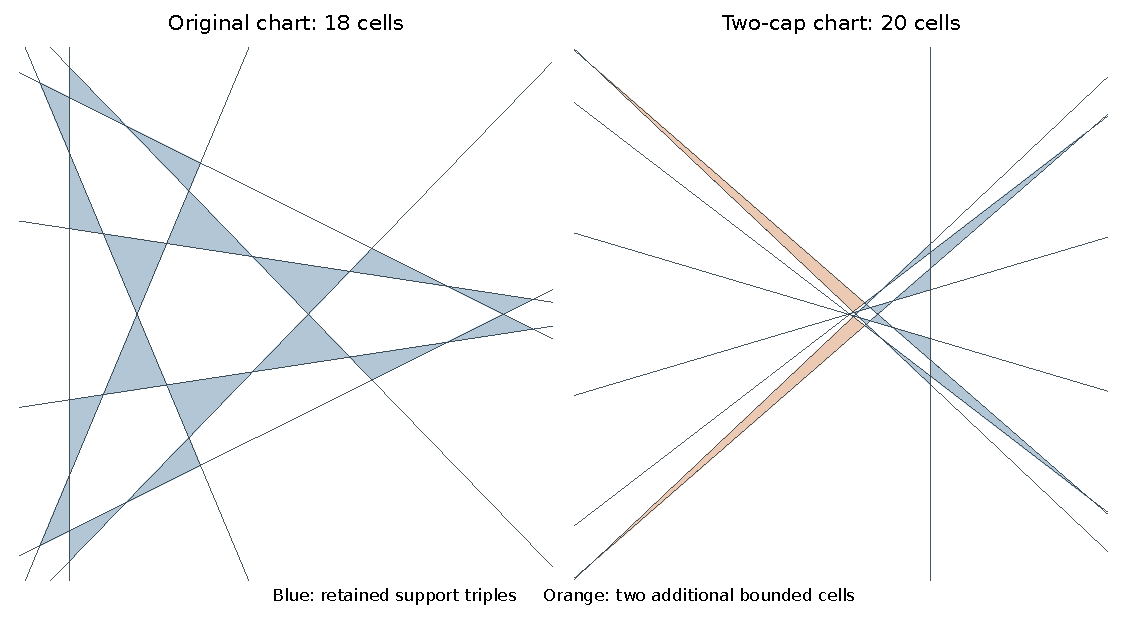
\includegraphics[width=.74\linewidth]{affine-chart.pdf}
\caption{Exact rational illustration of the two-cap change at $n=9$: 18 old cells survive and two become bounded. This gives $\G(9)=20$, below the known optimum 21. The general theorem uses real trigonometric coordinates; panels are independently rescaled.}\label{j:fig-chart}
\end{figure}

\begin{proof}[Proof of Theorem~\ref{j:main}]
For even orders use the shifted phase. If $n$ is odd and not divisible by three, $\B(n)+1=\floor{n(n-3)/3}+2$; use one cap. For odd multiples of three at least nine use two caps. A triangle handles $n=3$. The residue calculation gives the stated gains.
\end{proof}
The exact remaining gap is
\begin{equation}\label{j:gap}
 U_{\mathrm T}(n)-\G(n)
 =\floor{n/3}+\mathbf1_{n\equiv2\ (3)}-1-(n\bmod2),\qquad n\ge4.
\end{equation}
This is an independent construction at each order, not a successor chain from an arbitrary optimal seed.

\section{Exterior extensions and their boundary resource}
\label{jext:section}

Exterior addition has precedents in BBL and Blanc~\cite{bbl2008,blanc2011}.
The contribution here is an explicit geometric certificate, a quantitative
defect formulation for both parities, and an obstruction to repeatedly
demanding the full gain proposed in March~\cite{zarzuelo2026}.

Let $A$ be a simple $n$-line arrangement, $n\ge3$, with equations $f_i=0$ and
vertices $p_{ij}$.  A linear functional $w$ is admissible if it is nonzero
on every line direction.  At $p_{ij}$ choose support directions $u_i,u_j$
with $w(u_i)=w(u_j)=1$.  Call the pair \emph{visible} if, for every old
line $f_k=0$, the numbers
\[
 f_k(p_{ij}),\quad Df_k(u_i),\quad Df_k(u_j)
\]
have one common weak sign.  This condition certifies an empty unbounded
wedge using only old data.

\begin{theorem}[Verified exterior realization]
\label{jext:visible}
If $A$ contains $T$ distinct certified triangles and $c$ distinct pairs
visible from an admissible $w$, adjoining $w(x)=H$, where
$H>\max_{i<j}w(p_{ij})$, gives a simple arrangement with at least $T+c$
triangles.
\end{theorem}
\begin{proof}
The new line is nonparallel to every support, misses all old vertices,
and lies beyond every old bounded cell.  Thus simplicity and old triangles
are preserved.  A visible pair has new vertices
$p_{ij}+(H-w(p_{ij}))u_i$ and $p_{ij}+(H-w(p_{ij}))u_j$.
Their affine evaluations are
$f_k(p_{ij})+(H-w(p_{ij}))Df_k(u)$, so all three vertices have one weak
sign against every old line.  The triangle is nondegenerate and empty.
Distinct pairs give distinct new support triples, all containing the
new line and hence distinct from the old triples.
\end{proof}
This is \proofref{Kobon/Exterior.lean}{164}{\lean{Exterior.extension}}, a real-coordinate Lean theorem with
no parity restriction or assumed future count.

Write $T=t(A)$, $d=n(n-2)-3T$, and let $b$ count unbounded two-sided cells.
The quantity $d$ counts unused bounded elementary segments: a segment
in a simple arrangement supports at most one triangle.

\begin{theorem}[Actual boundary-defect extension]
\label{jext:defect}
For $n\ge3$, define
\begin{equation}
 g(n,T)=\ceil{\frac{n-1}{2n}\max\{3,\,3T-n(n-3)\}}.
 \label{jext:gain}
\end{equation}
Then $\Ks(n)\ge T$ implies $\Ks(n+1)\ge T+g(n,T)$.
\end{theorem}
\begin{proof}
There are $2n$ free rays, of which $2b$ belong to wedges.  At an unpaired
ray's endpoint $L\cap M$, both incident segments of $M$ are bounded.
They cannot both support triangles, since those triangles would share
the unique bounded segment of $L$ starting there.  Charge this ray to
an unused segment of $M$.  Each unused segment receives at most two
endpoint charges, giving $b+d\ge n$.  Convex-hull vertices of the finite
intersection set supply at least three wedges, so $b\ge\max\{3,n-d\}$.

The two rays of a wedge are consecutive in cyclic direction order.
Among the $2n$ admissible normal sectors, each wedge is visible in
exactly $n-1$: positivity selects $n$ consecutive oriented directions.
Thus some sector sees at least $\ceil{(n-1)b/(2n)}$ wedges.  Apply
Theorem~\ref{jext:visible}.  The expression is nondecreasing in $T$,
so a lower count can replace the witness's actual count.
\end{proof}
This is now an end-to-end real-geometric Lean theorem:
\proofref{Kobon/OpenMathEveryOrderExtension.lean}{45}{\lean{successor}}
extracts terminal rays, boundary wedges and admissible sectors from the
supplied simple witness. The supporting-point and sector proofs introduce
no convex-hull or visibility oracle. The earlier formula~\eqref{jext:gain}
is unchanged; its previously ordinary extraction steps are completed.
For $d=n(n-2)-3T$, its exact closed form is
\begin{equation}\label{jext:closed-gain}
 g(n,T)=\min\!\left(\floor{n/2},
 \ceil{\frac{\max\{3,\max(0,n-d)\}}2}\right).
\end{equation}
See \proofref{Kobon/OpenMathExtensionFormula.lean}{56}{\lean{closed_form_successor}}.

If $n=2m+1$ and $d\le2$, then $b\ge2m-1$.  Averaging forces at least
$m$ visible wedges, since
$2m(2m-1)>(4m+2)(m-1)$; no sector can contain more than $m$ disjoint
ray pairs. Hence every such odd input admits the full gain $m$.
For either parity the exact full-gain test is that some sector contains
$\floor{n/2}$ wedge pairs. The deficit rule iterates through both parities:
set $T_0=T$ and $T_{k+1}=T_k+g(n+k,T_k)$. Then $\Ks(n+k)\ge T_k$
for every $k\ge0$, by
\proofref{Kobon/OpenMathEveryOrderExtension.lean}{82}{\lean{infinite_quantitative_extension}}.
For $n\ge4$ every step gains at least two triangles. Numerical improvements
require suitable seeds; this iteration need not beat $\G$.

Repeated exterior additions have a finite boundary resource.  If $b_r$
is the wedge count and $c_r$ the gain, each new triangle consumes an
old wedge.  No new free ray appears at an old vertex, and new wedges
can use only the two free rays of the added line.  Therefore
\begin{equation}
 b_{r+1}+c_r\le b_r+2,\qquad
 \sum_{j<r}c_j\le b_0+2r-3.
 \label{jext:budget}
\end{equation}
Quadratically accumulating full gains cannot continue indefinitely.
For the saved $49:767$ seed, $b_0=47$; gains $24$ and $25$ in two
exterior steps would leave at most two wedges, contradicting $b\ge3$.
This does not refute a recurrence for maxima using reconstruction.

One recorded exterior chain has gains $24,23,2,2$, giving
$49{:}767\to50{:}791\to51{:}814\to52{:}816\to53{:}818$.
Its capacities describe those arrangements, not upper bounds for $\K$.
The companion manuscript plots the exact resource evolution.


Conditionally, $F(n+1)\ge F(n)+\floor{n/2}$ yields
\[
 F(n)\ge F(s)+\floor{(n-1)^2/4}-\floor{(s-1)^2/4}.
\]
The recurrence remains unproved for $\K$.  Nevertheless its $49$-seed
numerical target is independently unconditional:
\begin{equation}
 \K(n)\ge\floor{(n-1)^2/4}+191\qquad(n\ge49).
 \label{jext:49}
\end{equation}
Lean proves this from the finite 49/50 witnesses and the classical
baseline for $n\ge51$; it does not construct a nested full-gain chain.

\section{Completed recursive families and a total envelope}
\label{jfam:section}

The geometric doubling mechanism belongs to BBL~\cite{bbl2008}. A compatible seed supplies a tangent grid, simplicity, consecutive axis caps, positive central apex and certified triangle list. A visible seed additionally supplies an admissible normal and rightmost boundary pair.

\begin{theorem}[Verified BBL step]\label{jfam:doubling}
Let $q=4r\ge20$, $0<\varepsilon<\tan(\pi/(2q))$, and $t_j=\tan(j\pi/q)$. Take $Y_0:y=0$ and $L_j:y=m_j(x-a_j)$ on
\[
 (a_j)=(-t_{q/2-1},\ldots,-t_1,-\varepsilon,\varepsilon,t_1,\ldots,t_{q/2-1}).
\]
If these lines are simple, all $q-1$ axis caps are triangular, the central apex is positive and $T$ distinct triangles are certified, then $\Ks(2q+1)\ge T+q^2$.
\end{theorem}
\begin{proof}[Geometric mechanism]
For $\beta_i=-\pi/2+(i+1/2)\pi/q$, add
$y=\kappa(\sin(2\beta_i)+\delta\cot\beta_i)(x-\tan\beta_i)$.
Choose $\delta>0$, then $\kappa>0$, sufficiently small. Exact crossing order yields $2\binom{q+1}{2}-q=q^2$ mixed triangles. Old triangles off $Y_0$ persist, alternating caps replace its noncentral triangles, and the central triangle survives. The step returns the same geometric invariants, after actual support relabelling. A visible seed also retains projection order and boundary data.
\end{proof}

The eleven-line realization has reciprocal slopes
$(15,-2,14,1,4,-4,5,-3,12,-5)/10$ and, on $0<\varepsilon\le10^{-5}$, 32 triangles, nine caps and five visible pairs. Its count comes from a Honma-based input~\cite{savchuk2025}. A separate 21-line uniform seed has 132 triangles, 19 caps and ten visible pairs and starts the $r\ge5$ induction.

\begin{theorem}[Retained infinite families]\label{jfam:recursive}
For $t\ge0$, put $q=10\cdot2^t$ and $T_q=(q^2-4)/3$. Then
\begin{equation}\label{jfam:families}
 \Ks(q+1)\ge T_q,\qquad \Ks(q+2)\ge T_q+q/2.
\end{equation}
\end{theorem}
\begin{proof}
Uniform availability on some positive parameter interval survives every step. Starting with $(r,T,V)=(5,132,10)$, the actual transformation
$(r,T,V)\mapsto(2r,T+(4r)^2,V+2r)$
gives the displayed counts and $V=q/2$. The exterior theorem supplies the even companion. The eleven-line seed covers $t=0$. The interval may shrink with depth; a common positive interval for all depths is not claimed.
\end{proof}

\begin{theorem}[One-triangle simple windows]\label{jfam:windows}
For the same $q$,
\[
 T_q\le\Ks(q+1)\le T_q+1,\qquad
 T_q+q/2\le\Ks(q+2)\le T_q+q/2+1.
\]
\end{theorem}
\begin{proof}
Apply the actual simple bounds of Section~\ref{jup:section}; their floors are $T_q+1$ and $T_q+q/2+1$.
\end{proof}
The upper proofs use standard axioms. Existence inherits four finite native checks for the odd source and six for its even companion. This is a simple-model window; multiple intersections remain allowed in $\K$.

\begin{theorem}[Compatible 61-line orbit]\label{jfam:61}
For every $t\ge0$, put $q=60\cdot2^t$. Actual simple arrangements give
\begin{equation}\label{jfam:61-formula}
 \Ks(q+1)\ge1200\,4^t-10,\qquad
 \Ks(q+2)\ge1200\,4^t+30\,2^t-11.
\end{equation}
Their gaps to the respective simple upper floors are nine and ten.
\end{theorem}
\begin{proof}
A reciprocal-slope refit of Rohith Poola's OpenMath input~\cite{poola2026} preserves 1190 triangles and 59 axis caps for every real $0<\varepsilon\le10^{-8}$ on the actual tangent60 grid. Exact tangent enclosures and finite sign checks establish simplicity and all seed hypotheses. A further cap-cone mutation supplies 29 visible pairs, including the required boundary pair. BBL iteration gives $V_t=30\cdot2^t-1$, and exterior realization gives the even formula. See
\proofref{Kobon/OpenMathConstructionParetoFamily61.lean}{48}{\lean{odd_family}} and
\proofref{Kobon/OpenMathConstructionParetoFamily61.lean}{51}{\lean{even_family}}.
\end{proof}
Poola supplied the finite count 61:1190; BBL supplied doubling. The uniform compatible refit and 29-pair improvement are the present developments, with seven explicit finite native roots in the even proof. The earlier 28-pair seed remains preserved; its even count is one smaller at every depth. At 62 lines the new 1219 is below the retained $\G(62)=1220$. For $t\ge1$, the odd/even gains over $\G$ are $20\cdot2^t-11$ and $10\cdot2^t-11$: for example $121:4790$, $122:4849$, $241:19190$, $242:19309$. These are repository comparisons, without absolute numerical-priority claims.
\begin{figure}[tb]
\centering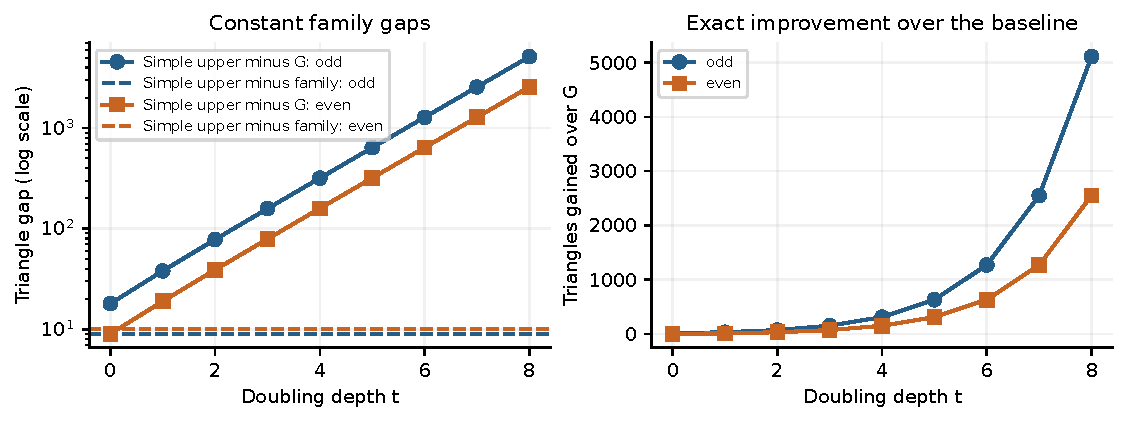
\includegraphics[width=.96\linewidth]{new-family61-gaps.pdf}
\caption{Exact formulas for $q=60\cdot2^t$, $0\le t\le8$. Left: the simple upper floors $U_{\rm T}(q+1)$ and $U_{\rm e}(q+2)$ minus the new odd/even counts remain nine/ten; the corresponding gaps to $\G$ grow. The vertical axis is logarithmic. Right: new counts minus $\G$, equal to $20\cdot2^t-11$ and $10\cdot2^t-11$. The even gain is $-1$ at $t=0$, so the envelope retains 1220 at order 62. These upper comparisons concern simple arrangements.}\label{jfam:61-gaps}
\end{figure}

\begin{corollary}[Completed known orbits]\label{jfam:known}
The compatible seeds in Table~\ref{jfam:orbits} give unconditional odd/even Lean families. Both branches attain their classical simple upper floors.
\end{corollary}
\begin{table}[tb]
\centering\small
\begin{tabular}{@{}rrll@{}}
\toprule
Seed & $q$ & Count at $q+1$ & Count at $q+2$\\\midrule
$33:341$ & $32\cdot2^t$ & $(1024\,4^t-1)/3$ & odd count $+16\cdot2^t$\\
$37:431$ & $36\cdot2^t$ & $432\,4^t-1$ & odd count $+18\cdot2^t$\\
$49:767$ & $48\cdot2^t$ & $768\,4^t-1$ & odd count $+24\cdot2^t$\\
\bottomrule
\end{tabular}
\caption{Formal completion of known numerical orbits: Forge--Ram\'irez Alfons\'in, Parpalak--Utkin/Blanc and BBL, respectively~\cite{forge1998,parpalakutkin2026,blanc2011,bbl2008}.}\label{jfam:orbits}
\end{table}
The 33/49 finite seed checks were unfinished in the 3 October release; they are now discharged. The 37 orbit uses a compatible refit of Poola's $37:431$ input~\cite{poola2026} and the actual odd deficit-two successor, requiring no additional visibility check. The simple counts $38:449$ and $50:791$ are below retained nonsimple witnesses $38:450$ and $50:792$. The corrected five-line seed (five triangles, three caps, two visible pairs on $0<\varepsilon\le10^{-5}$) and the external uniform 19:107 seed check (17 caps on $0<\varepsilon\le10^{-3}$) retain their earlier evidence and attribution. The inherited odd families at $q=4\cdot2^t$ and $q=18\cdot2^t$ count $(q^2-1)/3$ and $q^2/3-1$, respectively; their simple even companions add $q/2$ by the now-verified deficit-two rule. The table completes the specified later tails in Lean.

Let $C(n)$ be the largest saved finite count, or zero. Retain
\begin{equation}\label{j:envelope}
 L(n)=\max\{\G(n),C(n)\}\le\K(n).
\end{equation}
Let $R(n)$ select the $q=10\cdot2^t$ odd/even counts, and vanish otherwise.
\begin{theorem}[Retained and enlarged envelopes]\label{j:new-envelope}
For every natural $n$,
\begin{equation}\label{j:new-envelope-formula}
 \K(n)\ge H(n):=\max\{L(n),R(n)\}\ge L(n).
\end{equation}
This is strict at $10\cdot2^{t+5}+1$ and $10\cdot2^{t+5}+2$. The enlarged executable envelope
\begin{equation}\label{j:portfolio}
 \K(n)\ge P(n):=\max\bigl(H(n),\max_{0\le t\le n}
 \{F_{33}(n,t),F_{37}(n,t),F_{49}(n,t),F_{61}(n,t)\}\bigr)
\end{equation}
retains $H$ pointwise, where candidates vanish away from their specified odd/even orders.
\end{theorem}
\begin{proof}
Take the finite maximum of actual witnesses. The old catalog stops at order 195. Beyond that,
\begin{equation}\label{j:new-gains}
 T_q-\G(q+1)=\floor{q/3}-2,\quad
 T_q+q/2-\G(q+2)=q/2-\floor{q/3}-2,
\end{equation}
both positive from $q=320$. The new maximum is
\proofref{Kobon/OpenMathConstructionEnvelope.lean}{97}{\lean{all_n}};
\proofref{Kobon/OpenMathConstructionEnvelope.lean}{100}{\lean{previous_le}}
proves retention. Its leading quadratic quality is inherited.
\end{proof}
The old checkpoints $81:2132$, $82:2172$, $161:8532$, $162:8612$, and existence bounds $321:34132$, $322:34292$, $641:136532$, $642:136852$ remain. Their gains at 321/322 are 104/52, at 641/642 are 211/105. Existing small-order certificates may dominate the simple families, including $12:38$, $21:133$, $22:143$, $41:533$ and $42:553$. No new theorem retroactively certifies unfinished archived coordinate files.

\section{Actual incidence and component bounds}
\label{jup:section}

Here the $n\ge2$ real lines are pairwise nonparallel. Multiple points are allowed except in explicitly simple or all-triple statements. All counts refer to a finite injective family of certified triangular cells, which may be a subset of all cells. A \emph{core} is an intersection of multiplicity $r\ge3$. Put
\[
 q=\sum_{r\ge3}t_r,\quad I=\sum_{r\ge3}rt_r,\quad
 S=\sum_{r\ge3}r(r-2)t_r,\quad\delta=n(n-2)-3T.
\]
Let $h$ count lines meeting a core, $E$ bounded elementary segments, $U$ unused segments, and $D_1,D_2$ shared sides with one and two core endpoints. Actual geometry gives
\begin{equation}\label{jup:identity}
 E=n(n-2)-S,\quad3T=E-U+D_1+D_2,\quad
 \delta=S+U-D_1-D_2.
\end{equation}
It also gives $D_2+h\le I$, $D_2\le\binom q2$, and $2S-7I+15q\ge0$.

\begin{lemma}[Actual clean-line charging]\label{jup:clean}
For even $n\ge4$, $n-h\le2U+D_1$; hence
\begin{equation}\label{jup:budget}
 2\delta\ge n+2S-h-3D_1-2D_2.
\end{equation}
\end{lemma}
\begin{proof}
A clean line has $n-1$ crossings. Select bounded transverse segments on one common side. If all had triangle degree one, their triangle bases would partition the crossings into pairs, contradicting odd cardinality. Thus some chosen segment is unused or shared. Ordinary-endpoint uniqueness permits at most two charges on an unused side and one on a one-core shared side. The choices and fibers are extracted in Lean.
\end{proof}
Nonparallelism is used to obtain transverse intersections; this statement is distinct from the completed exterior-ray charging of Section~\ref{jext:section}.

\begin{theorem}[Formal classical simple bounds]\label{jup:simple}
Every simple certificate satisfies $3T\le n(n-2)$, and for even $n\ge4$, $6T\le n(2n-5)$.
\end{theorem}
\begin{proof}
The core is empty, so $\delta=U\ge0$; the even charge budget gives $2U\ge n$.
\end{proof}
These retain the classical attribution, including Blanc's even bound~\cite{blanc2011}.

\begin{lemma}[Extracted local fans]\label{jup:fan}
At an $r$-fold core let $a,d$ be the ordinary-ended and core-ended shared-ray degrees. Then $a\le2r-3$ and $3a+d\le6r-6$. Equality $a=2r-3$ forces every sector triangular and $d=3$. In particular $d\le2$ implies $a\le2r-4$, and
\begin{equation}\label{jup:sharp-fan}
 3a+d\le6r-8+2e_v,
\end{equation}
where $e_v$ indicates $a=2r-3$.
\end{lemma}
\begin{proof}
A run of $r-1$ ordinary-ended shared rays would force an opposite support through the center. Cyclic window counting bounds $a$; a missing sector improves it by one. The canonical ray order, antipodes, endpoint correspondence and neighboring triangle matches are now extracted from the actual arrangement, completing the former local-interface gap.
\end{proof}
A finite support extreme cannot carry the full exceptional fan; two exceptional full triple fans cannot be adjacent. Summation now proves
\begin{equation}\label{jup:exceptional}
 2\delta\ge n+2S-7I+8q+D_2-2\sum_v e_v
 \qquad(n\ge4\text{ even}),
\end{equation}
in \proofref{Kobon/UpperOpenMathGlobalFans.lean}{204}{\lean{certificate_defect_even}}, without a supplied fan premise.

\begin{theorem}[Retained restricted estimates, now extracted]\label{jup:upper}
For even $n\ge4$ and nonparallel arrangements,
\begin{equation}\label{jup:weighted}
 2\delta\ge n+\sum_{r\ge3}(2r^2-11r+6)t_r.
\end{equation}
If there are at most two cores,
\begin{equation}\label{jup:two-core}
 T\le\floor{n(n-5/2)/3}+1.
\end{equation}
The zero/one-core defects satisfy $\delta\ge n/2$ and $\delta\ge n/2-1$. With at most three cores, $T\le\floor{n(2n-5)/6}+2$.
\end{theorem}
\begin{proof}
Sum the fan bounds and use~\eqref{jup:budget}. With at most three cores each core has $d\le2$, giving $D_1\le2I-4q$. Core-path incidence and $D_2\le\binom q2$ give the stated bounds, with integer parity rounding. Actual two/three-core wrappers are
\proofref{Kobon/UpperOpenMathBoundaryBudgets.lean}{137}{\lean{certificate_two_core_upper}} and
\proofref{Kobon/UpperOpenMathBoundaryBudgets.lean}{128}{\lean{certificate_three_core_upper}}.
\end{proof}
The two-core bound is attained at $8,14,26,50$ lines by attributed $15,54,204,792$ witnesses~\cite{maiorana2026,parpalakutkinGallery2026}. Multiplicities at least five make the old weight nonnegative; triple and quadruple weights remain negative.

For the new component estimates, join cores exactly when a shared elementary side joins them. Let $c$ count components, including isolated cores, and let $\Sigma=\sum_{r\ge4}r(r-4)t_r$. Let $A$ count triple cores of type $(a,d)=(2,4)$ and $B_s$ count those of type $(1,5)$ in component $s$.

\begin{theorem}[Mixed-multiplicity component penalty]\label{jup:mixed}
For arbitrary core multiplicities, degrees and component sizes,
\begin{equation}\label{jup:mixed-formula}
 \delta+A+\sum_s\ceil{B_s/2}\ge U+c+\Sigma.
\end{equation}
If every core degree is at most three, or every component has at most five cores, the corrections disappear: $\delta\ge U+c+\Sigma$.
\end{theorem}
\begin{proof}[Charging and escape]
Actual cap-neighbor maps pay extremal sources against poor recipients. Higher multiplicities supply quadratic surplus. A finite support extreme and the geometric exclusion of closed balanced triple cycles force a positive unit in each component after the displayed corrections. Connected-component partitions and integer rounding give
\proofref{Kobon/UpperOpenMathMixedCurvatureBound.lean}{41}{\lean{certificate_mixed_curvature_component_bound}}.
The correction-free cases use
\proofref{Kobon/UpperOpenMathMixedDegreeThree.lean}{158}{\lean{certificate_mixed_degree_three_component_bound}} and
\proofref{Kobon/UpperOpenMathMixedFiveCoreComponents.lean}{96}{\lean{certificate_mixed_five_component_bound}}.
\end{proof}

In the all-triple class, a \emph{marked port} is a core-ended shared ray whose two immediate neighboring rays are ordinary-ended shared rays. Let $A_0$ count unmarked $(2,4)$ cores, $B=\sum_s B_s$, $E_3$ count $a=3$ cores, $P_{21}$ count $(2,1)$ cores, $N_{12}$ count $(1,2)$ cores, and $M_{22}$ count marked $(2,2)$ cores. Subscripts $s$ restrict these counts to a component.

\begin{theorem}[All-triple refinements]\label{jup:triple}
Without degree or component-size restrictions,
\begin{equation}\label{jup:m22}
 2\delta+B\ge2U+3(E_3+P_{21})+N_{12}+M_{22}.
\end{equation}
A separately completed component estimate is
\begin{equation}\label{jup:hybrid}
 \delta\ge U+\sum_s\max\!\left(
 1-A_s-\ceil{B_s/2},
 \ceil{\frac{3E_s+3P_s+N_{12,s}-B_s}{2}}\right),
\end{equation}
where $A_s$ counts the $A_0$ cores in $s$. If each component satisfies
$B_s+1\le3E_s+3P_s+N_{12,s}$, then $\delta\ge U+c$.
\end{theorem}
\begin{proof}[Actual recipient exclusions]
An unmarked full $(2,4)$ source has antipodal ordinary rays. Actual side matching excludes source adjacency and limits their recipient incidence. A $(1,3)$ or $(1,2)$ recipient has at most one such source neighbor; a $(2,1)$ recipient has none. These geometric exclusions remove the former double-recipient correction. Marked and incoming antipodal-source edges are disjoint, so $m+x\le d$ locally; at a marked $(2,2)$ core this retains a further unit. The global root is
\proofref{Kobon/UpperOpenMathM22Curvature.lean}{117}{\lean{certificate_m22_source_free_defect_bound}};
the component root is
\proofref{Kobon/UpperOpenMathClosedN12Curvature.lean}{282}{\lean{certificate_n12_source_free_hybrid_component_defect}}.
The last implication follows by rounding, and is independently checked.
\end{proof}
All structural endpoints use only standard logical axioms. Equation~\eqref{jup:m22} includes $M_{22}$ globally; no component $M_{22}$ refinement is claimed. Earlier paid-component and half-curvature bounds remain proved and are dominated by the retained component portfolio. Mixed forests also satisfy $\delta\ge U+c+\sum_{r\ge4}(r(r-4)+1)t_r$; degree-four mixed components retain only the $A$ correction. The broad assertion that exact Tamura equality forces simplicity already appears in Cl\'ement--Bader~\cite{clementbader2007}; our sufficient-class corollaries do not claim its first discovery. Local cap and kite mechanisms also retain OpenMath-source credit~\cite{srirangam2026}.

The residual $B$ correction and the profile hypothesis cannot be dropped. General strict component positivity, the all-triple token targets $C_{\rm end}\ge2D_1$ and $n\le2U+D_1+R_c+2$, and a new unrestricted even numerical bound remain open. Here $C_{\rm end}$ counts nonshared core-end incidences and $R_c$ unbounded core rays. The safe extracted all-line budget is $n\le2U+2D_1+C_{\rm end}$ for even $n\ge4$ all-triple arrangements.

The six-line triangle-and-medians arrangement $x=0$, $y=0$, $x+y=3$, $x-y=0$, $2x+y=3$, $x+2y=3$ retains six cells and six shared radial sides at $(1,1)$, with $a=d=3$. Its exact certificate challenges only a literal local incidence reading of a shared-pair assertion~\cite{clementbader2007}, not the final upper theorem.
\begin{figure}[tb]
\centering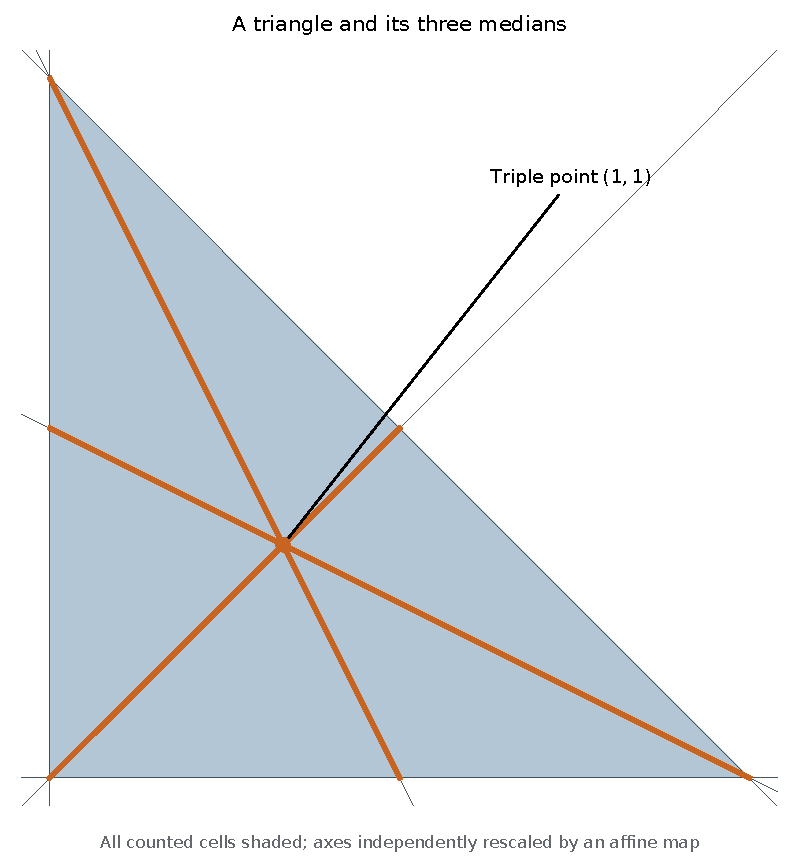
\includegraphics[width=.36\linewidth]{shared-fan.pdf}
\caption{The retained verified shared-fan example. Separating ordinary-ended and core-ended sides is essential.}\label{jup:figure}
\end{figure}

\begin{proposition}[Exact translation surgery]\label{jup:surgery}
For sufficiently small positive parallel translation of one line in a finite nonparallel arrangement, triangle predicates are determined by affine determinant germs. With the exact sets of lost and born support triples,
\begin{equation}\label{jup:surgery-identity}
 T(\varepsilon)+\#\mathrm{lost}=T(0)+\#\mathrm{born}.
\end{equation}
\end{proposition}
This follows from simultaneous sign stability and
\proofref{Kobon/OpenMathTranslationCounting.lean}{98}{\lean{translated_birth_loss_identity}}.
Exactly one concurrent supporting triple gives one birth, with retention requiring global conditions. Loss is not a half-plane triangle count~\cite{liuDesingularization2026}: a four-line witness remains at two cells despite zero proposed half-plane loss. For the six lines
$y=0$, $x-y=0$, $x+y=0$, $x+2y=3$, $-2x+y=2$, $x+4y=-4$,
replacing $y=0$ by $y=\varepsilon$ or $y=-\varepsilon$ gives seven or four cells for every $0<\varepsilon<1/100$, from six initially. The downward resolution breaks three old triangles and creates one. These standard-axiom interval proofs refute a general loss cap of two. Earlier Maiorana $14:54$ resolutions $52,52,53,52$, and 132 gallery resolutions with best nearby simple counts $14,51,114,203,313,448,791$ at orders $8,14,20,26,32,38,50$, remain exact external diagnostics, not bounds on every simple arrangement.

\section{Finite results, exact obstructions, and verification}\label{j:verification}

The release retains 138 coordinate identities, 104 simple, with original credits. Table~\ref{j:finite} preserves the individual historical inequalities and all eleven later affine materializations. The companion catalog lists every input and its source.
\begin{table}[tb]
\centering\small
\begin{tabular}{@{}llp{.33\linewidth}@{}}
\toprule
Order(s) & Certified counts, in order & Role\\\midrule
$28,30,34$ & $238,275,357$ & Historical inequalities\\
$44$ & $608$ & Simple optimum\\
$39,47,48$ & $470,691,721$ & Earlier retained count plus one\\
$51,53,54,55$ & $818,885,919,955$ & Earlier retained count plus one\\
$59,60,99,195$ & $1103,1141,3170,12482$ & Earlier retained count plus one\\
\bottomrule
\end{tabular}
\caption{Selected exact simple witnesses. The increases are relative to earlier project certificates, not asserted global records. All orders 3--60 and all 138 coordinate identities are in the companion evidence.}\label{j:finite}
\end{table}

The March-associated $28{:}238$, $30{:}275$, $34{:}357$ inequalities now have independent certificates; the archived extension proof remains incomplete~\cite{zarzuelo2026,oeisA006066}. Earlier literature overlaps are explicit: $30{:}275$ is in BBL, and $34{:}357$ follows from the older perfect 33-line construction and exterior addition~\cite{bbl2008,forge1998}. The exact $43{:}587\to44{:}608$ construction combined with the now-formal simple upper theorem gives $\Ks(44)=608$, not $\K(44)=608$. The earlier proposed value $q^2/3+q+1$ at $n=q+3$, $q=6\cdot2^t$, is superseded by $\G(q+3)=q^2/3+q+2$.

Two independent rational counters support the finite catalog. Reproduced external inputs include all fifteen Maiorana $14{:}54$ configurations and ten Parpalak--Utkin gallery witnesses, including $26{:}204$ and $50{:}792$~\cite{maiorana2026,parpalakutkinGallery2026}. Exact projective face censuses for the saved 81- and 161-line examples equal 2132 and 8532, their bounded counts: a chart change alone cannot improve these two fixed arrangements.

\paragraph{A prescribed-grid obstruction.}
In reciprocal coordinates $x-v_i y=a_i$, required orientation signs become strict linear inequalities in the $v_i$. Positive linear dependencies certify infeasibility. Lean proves this Farkas-type soundness principle and the exact coefficient field
\[
 t=\tan(\pi/20),\qquad t^4-4t^3-14t^2-4t+1=0,\qquad3/20<t<17/100,
\]
including all nine positive grid tangents as power-basis expressions.
\begin{proposition}\label{j:obstruction}
The ten specified orientation signs linked in \proofref{Kobon/BBLGridObstruction.lean}{263}{the exact obstruction statement} cannot occur on the prescribed 20-intercept tangent grid, for any real $\varepsilon$ and arbitrary real reciprocal slopes.
\end{proposition}
This representative obstruction is fully in Lean with standard axioms. A separate exact verifier checks 3,765 polynomial dependencies and 15,060 reflected/reoriented variants, covering all $236\cdot21=4,956$ supplied Euclidean-class/distinguished-support cases for $0<\varepsilon<1/2{,}000{,}000$. The input classification and its completeness are attributed to Parpalak--Utkin~\cite{parpalakutkinEnumeration2026}; their enumeration is not rerun or formalized here. Subject to that external classification, the corpus excludes a perfect 21-line seed on this specific saturated grid and interval. The earlier 18-projective-representative scan omitted affine charts and has been replaced by this corrected coverage. An exact external interval calculation also proves radius-$10^{-3}$ intercept robustness for the representative's eleven used intercepts. Other grids and larger seeds remain possible.

\paragraph{Uniform seed completion and bounded searches.}
The 49-line seed's exact rational reciprocal slopes have denominator $10^{10}$ on the actual 48-intercept tangent grid. On $0<\varepsilon\le1/100$ it has 767 triangles, 47 caps and 24 visible pairs from $(1,-2)$, with positive central apex. The former finite Lean bottleneck is resolved without changing its geometric predicates or interval. Both 33/49 families in Table~\ref{jfam:orbits} are therefore unconditional; for reference the latter gives
\begin{equation}\label{j:exact49}
 768\,4^t-1\text{ at }48\cdot2^t+1,\qquad
 768\,4^t+24\cdot2^t-1\text{ at }48\cdot2^t+2.
\end{equation}
Sound Boolean reflection and memoized coefficient arrays made the large finite checks feasible. True tangent enclosures and the real-geometric bridges remain standard-axiom proofs; finite native checks retain their disclosed compiler/runtime trust.

Earlier bounded searches found no numerical record: deletion, mixed-integer line selection, singular insertions and straightening are logged with their limits. For example, all 9,180 tested 17-line vertex-pair chords reached at most 93 triangles at order 18; 407,253 tested 43-line pairs reached 607 at order 44. Two 39-line straightening searches certified 353 and 358 triangles, respectively; neither is a record or a nonstretchability result. These experiments motivate certificates and alternate grids, not impossibility claims.

\paragraph{Proof release and remaining work.}
The mathematical sources use Lean 4.31.0 and Mathlib~\cite{lean4,mathlib}. The 5--6 October research snapshot contains 638 active modules: 265 compiled in its incremental replay and 373 unchanged source/import closures reused from the verified baseline. Its whole-project axiom audit checks 9,058 declarations, 8,046 standard-only and 1,012 additionally depending on explicit finite native roots, with no admitted proofs or unapproved axioms. These are audit counts, not discoveries; incremental verification is distinguished from a clean build. Immutable source links and the final release evidence are listed in the companion result map.

Exact cap-cone searches proposed the 29-pair seed; whole-interval arithmetic and Lean replay supplied its proof. The corpus also disproves several tempting shortcuts: adjacent higher-order extremal fans exist, residual negative triple types need not be independent, and token rules valid in finite all-triple screens can fail with higher multiplicities. Those rational counterexamples and bounded negative searches remain attributed research evidence. The general positive component escape and the corrected all-triple even token trade-off remain open; the March full-gain recurrence for unrestricted maxima remains unproved. Larger compatible seeds and globally certified surgery remain constructive directions. The source, experiments and expanded manuscript~\cite{zarzueloRepository,zarzueloFull2026} preserve earlier work and the 5--6 October additions. Exact search, computer algebra and AI assistance contributed to the development; every promoted conclusion is tied to its stated proof evidence.

\section*{Result-to-proof index}\label{j:proof-index}

Immutable source anchors accompany the final mathematical revision.
\textbf{K} denotes standard Lean axioms; \textbf{N} also inherits explicit finite native checks; \textbf{P} denotes an ordinary manuscript argument; \textbf{E} denotes exact external computation. The
\href{https://github.com/alejandrozu/kobon-proof/blob/manuscripts-2026-10-07/manuscripts/2026-10-07/shared/proof_map.md}{complete result map}
retains every earlier claim and all 138 coordinate identities, and lists the new endpoints, hypotheses and release evidence.

\begingroup\small\renewcommand{\arraystretch}{0.96}
\setlength{\LTleft}{0pt}\setlength{\LTright}{0pt}
\begin{longtable}{@{}>{\raggedright\arraybackslash}p{.27\linewidth}>{\raggedright\arraybackslash}p{\dimexpr.73\linewidth-2\tabcolsep\relax}@{}}
\toprule
Result & Immutable source and scope\\\midrule
\endfirsthead
\toprule
Result & Immutable source and scope (continued)\\\midrule
\endhead
\midrule
\endfoot
\bottomrule
\endlastfoot
Theorem~\ref{j:main}; \eqref{j:G}, \eqref{j:gap} &
\proofref{Kobon/Universal.lean}{26}{All-order construction},
\proofref{Kobon/Universal.lean}{72}{gains},
\proofref{Kobon/Universal.lean}{90}{gap}: K.\\
Lemma~\ref{j:cell}; phase and caps &
\proofref{Kobon/Cells.lean}{486}{Sign-cell equality},
\proofref{Kobon/Cells.lean}{453}{disjointness},
\proofref{Kobon/ShiftedFurediPalasti.lean}{274}{phase},
\proofref{Kobon/FurediPalastiWrap.lean}{191}{one cap},
\proofref{Kobon/FurediPalastiTwoCaps.lean}{282}{two caps}: K; complement-component interpretation P.\\
Theorem~\ref{jext:visible} &
\proofref{Kobon/Exterior.lean}{164}{Exterior realization}: K from certified visible pairs.\\
Theorem~\ref{jext:defect}; \eqref{jext:closed-gain} &
\proofref{Kobon/OpenMathEveryOrderExtension.lean}{45}{Actual successor},
\proofref{Kobon/OpenMathExtensionFormula.lean}{56}{closed formula},
\proofref{Kobon/OpenMathEveryOrderExtension.lean}{82}{indefinite iteration},
\proofref{Kobon/OpenMathBoundarySuccessor.lean}{84}{odd deficit-two step}: K.\\
Resource \eqref{jext:budget}; target \eqref{jext:49} &
\proofref{Kobon/Iteration.lean}{105}{Conditional resource arithmetic}: K with geometric resource argument P;
\proofref{Kobon/AllN.lean}{504}{unconditional numerical target}: N, no full-gain chain.\\
Theorems~\ref{jfam:doubling}--\ref{jfam:windows} &
\proofref{Kobon/BBLDoubling.lean}{15}{BBL step},
\proofref{Kobon/BBLRecursiveSeed.lean}{61}{seed step},
\proofref{Kobon/BBLVerifiedFamilies.lean}{24}{odd},
\proofref{Kobon/BBLVerifiedFamilies.lean}{51}{even},
\proofref{Kobon/BBLFamilyOptimality.lean}{29}{odd window},
\proofref{Kobon/BBLFamilyOptimality.lean}{35}{even window}: N existence, K upper halves.\\
Theorem~\ref{jfam:61} &
\proofref{Kobon/OpenMathConstructionParetoFamily61.lean}{48}{Odd},
\proofref{Kobon/OpenMathConstructionParetoFamily61.lean}{51}{even},
\proofref{Kobon/OpenMathConstructionParetoFamily61.lean}{59}{one-unit improvement}: N existence; finite count credited to Poola.\\
Corollary~\ref{jfam:known}; Table~\ref{jfam:orbits} &
\proofref{Kobon/OpenMathConstructionForgeFamily.lean}{25}{33 odd},
\proofref{Kobon/OpenMathConstructionForgeFamily.lean}{28}{33 even},
\proofref{Kobon/OpenMathConstructionFamily37.lean}{54}{37 odd},
\proofref{Kobon/OpenMathConstructionFamily37.lean}{58}{37 even},
\proofref{Kobon/BBL49VerifiedFamilies.lean}{36}{49 odd},
\proofref{Kobon/BBL49VerifiedFamilies.lean}{48}{49 even}: N; simple optimality follows from K upper bounds.\\
Theorem~\ref{j:new-envelope} &
\proofref{Kobon/RecursiveEnvelope.lean}{51}{Retained envelope},
\proofref{Kobon/RecursiveEnvelope.lean}{73}{strict old gains},
\proofref{Kobon/OpenMathConstructionEnvelope.lean}{97}{new portfolio},
\proofref{Kobon/OpenMathConstructionEnvelope.lean}{100}{pointwise retention}: N witnesses, K comparisons.\\
Identity~\eqref{jup:identity}; Lemma~\ref{jup:clean}; Theorem~\ref{jup:simple} &
\proofref{Kobon/UpperEdgeInventory.lean}{345}{Defect},
\proofref{Kobon/UpperCleanCharging.lean}{100}{clean charge},
\proofref{Kobon/UpperSimpleOptimality.lean}{70}{simple floor},
\proofref{Kobon/UpperEvenSimpleOptimality.lean}{69}{even floor}: K.\\
Lemma~\ref{jup:fan}; Theorem~\ref{jup:upper} &
\proofref{Kobon/UpperOpenMathActualFans.lean}{197}{Actual fan extraction},
\proofref{Kobon/UpperOpenMathGlobalFans.lean}{204}{summed defect},
\proofref{Kobon/UpperOpenMathBoundaryBudgets.lean}{137}{two cores},
\proofref{Kobon/UpperOpenMathBoundaryBudgets.lean}{128}{three cores}: K, no supplied fan premise.\\
Theorem~\ref{jup:mixed} &
\proofref{Kobon/UpperOpenMathMixedCurvatureBound.lean}{41}{Mixed correction},
\proofref{Kobon/UpperOpenMathMixedDegreeThree.lean}{158}{degree three},
\proofref{Kobon/UpperOpenMathMixedFiveCoreComponents.lean}{96}{five-core components}: K.\\
Theorem~\ref{jup:triple} &
\proofref{Kobon/UpperOpenMathM22Curvature.lean}{117}{Global M22},
\proofref{Kobon/UpperOpenMathClosedN12Curvature.lean}{282}{component N12},
\proofref{Kobon/UpperOpenMathPositiveProfileComponents.lean}{43}{positive profile},
\proofref{Kobon/UpperOpenMathLocalPortBudget.lean}{10}{local port budget}: K, all cores triple.\\
Other component/parity results &
\proofref{Kobon/UpperOpenMathForestBudget.lean}{95}{Mixed forests},
\proofref{Kobon/UpperOpenMathMixedDegreeFour.lean}{169}{degree four},
\proofref{Kobon/UpperOpenMathOrdinaryGlobalCharge.lean}{146}{safe all-line charge}: K with displayed class hypotheses.\\
Proposition~\ref{jup:surgery} &
\proofref{Kobon/OpenMathTranslationCounting.lean}{98}{Birth/loss identity},
\proofref{Kobon/OpenMathFourLineResolution.lean}{59}{four-line classification},
\proofref{Kobon/OpenMathSixLineResolution.lean}{557}{seven cells},
\proofref{Kobon/OpenMathSixLineResolution.lean}{566}{four cells},
\proofref{Kobon/OpenMathSixLineResolution.lean}{579}{three old losses}: K real-parameter proofs.\\
Figure~\ref{jup:figure}; Table~\ref{j:finite} &
\proofref{Kobon/SharedFan.lean}{51}{Six shared sides}: K;
\proofref{verification/certificate-index.json}{1}{finite certificate index}: N where recorded.\\
Proposition~\ref{j:obstruction}; diagnostics &
\proofref{Kobon/BBLGridObstruction.lean}{263}{Tangent-grid sign obstruction}: K for the specified system; full 236-class corpus, intercept robustness, smoothing and bounded searches E.\\
\end{longtable}\par\endgroup

\begingroup
\small
\setlength{\bibsep}{3pt}
\bibliographystyle{plainnat}
\bibliography{references}
\endgroup
\end{document}
